\subsection{Kavicsos talajon helyben forgás}
A \ref{fig:Left_n50Right50a} megfigyelhető amint a robot kavicsos talajon differenciálisan fordul 60 másodpercen keresztül, ezalatt háromszor teljen körbefordul. A palyát tekintve a robot középontja elmozdul, az X tengelyen 0.22m-t és a Y tengelyen 0.6m-t.  Az oldalirányú mozgás a nem egyenlő surlodási erők miatt jön létre.
A fordulas közben a kerekek követik az előírt referencia szögsebességeket, amint az \ref{fig:Left_n50Right50x} ábrán is látható.
A frdulási szögsebesség 20 \degree/s, az X és Y tengelyen való sebesség elhanyagolható nagyságú de jelen van mivel a robot forgási közepontja elmozdul \ref{fig:Left_n50Right50b}.

A talajon levő 0.8-1.1cm átmérőjü kavicsok miat a surlodások is megváltoznak, az kereke oldalirányú surlodásai kissebbek lesznek, emiatt a robot könyebben fordul. A kavicsok hasonloképpen viselkednek a csapágyakban található gorgökhoz.
Abban az esetben ha a talajt a kavicsok nem teljes mértékben fedik be a \ref{fig:Left_n50Right50a} látható mozgáspálya keletkezik, azáltal hogy csak néha kerül a kerék alá a gördülékeny kavics.

\renewcommand{\nth}{2}
\renewcommand{\GlobalPath}{Meresek/Mozgasok/NormalMukodes/DiferencialisanHelybeKavicsos/}
\renewcommand{\secondImage}{*}



\begin{figure}[H]
  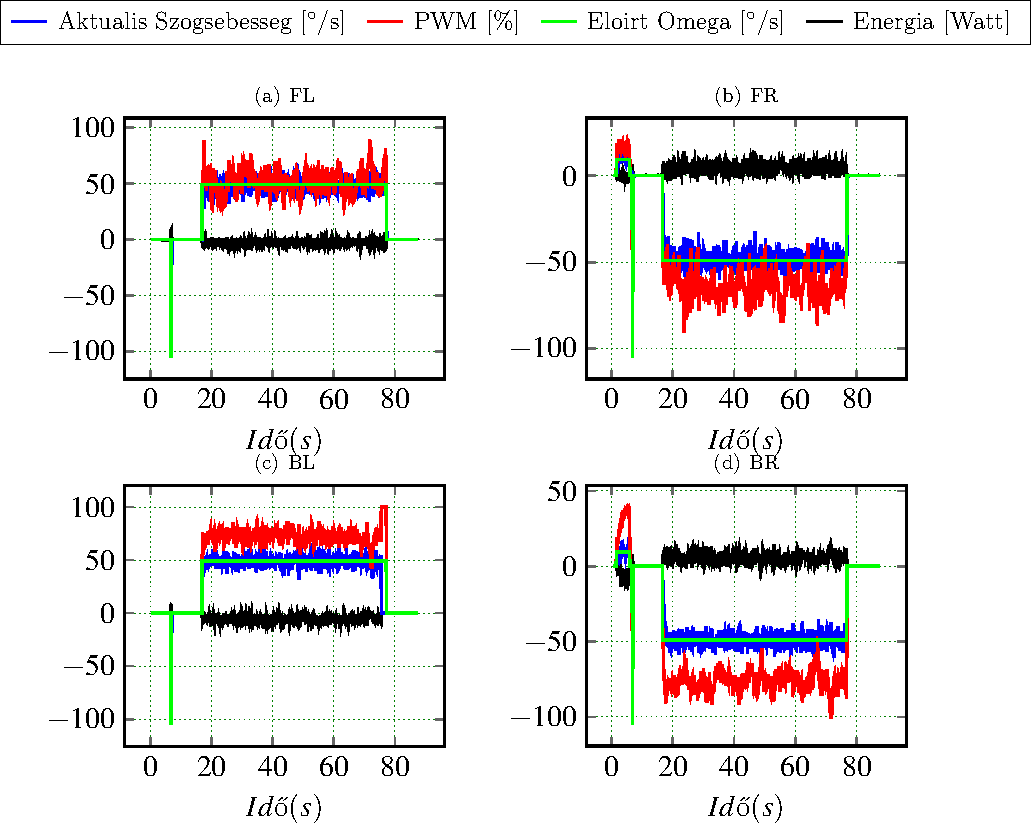
\includegraphics{tikz/Left_n50Right50x.pdf}
  \caption{$SSMR-4W$ típusú robot mozgása, tengelyekre bontva, ha a kerekszőgsebességek BL=FL=50\degree/s es a FR=BR=-50\degree/s}
  \label{fig:Left_n50Right50x}
\end{figure}


\begin{figure}[H]
  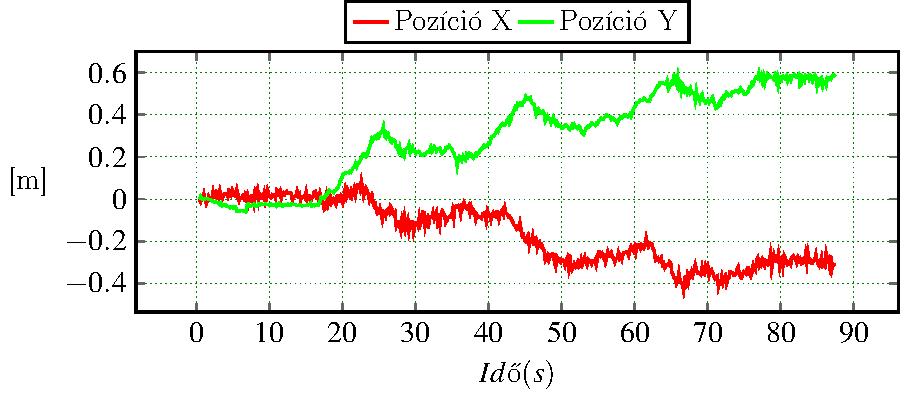
\includegraphics{tikz/Left_n50Right50a.pdf}
  \caption{$SSMR-4W$ típusú robot mozgása, ha a kerekszőgsebességek BL=FL=50\degree/s es a FR=BR=-50\degree/s}
  \label{fig:Left_n50Right50a}
\end{figure}


\begin{figure}[H]
  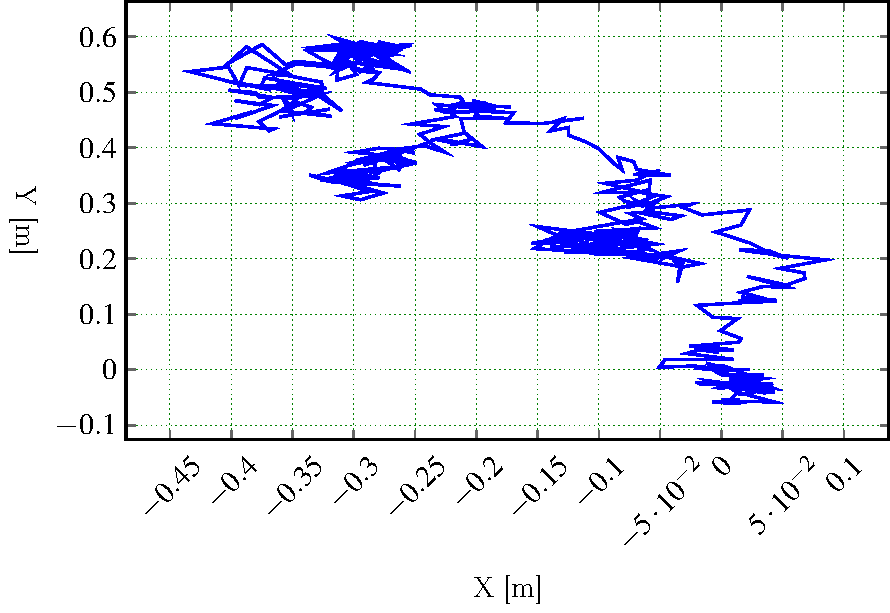
\includegraphics[scale=1]{tikz/Left_n50Right50b.pdf}
  \caption{$SSMR-4W$ típusú robot által leírt pálya, ha a kerekszőgsebességek BL=FL=50\degree/s és a FR=BR=-50\degree/s}
    \label{fig:Left_n50Right50b}
\end{figure}



\begin{figure}[H]
  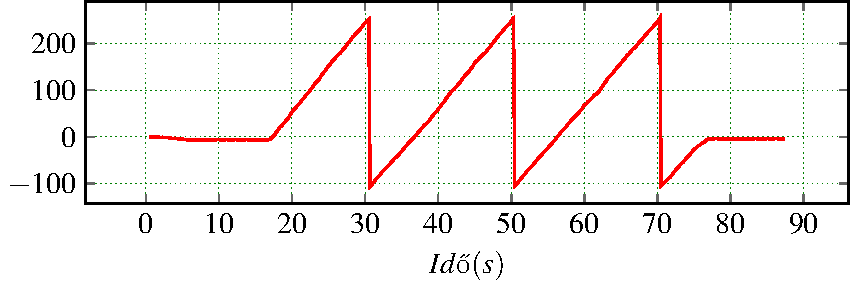
\includegraphics{tikz/Left_n50Right50c.pdf}
  \caption{$SSMR-4W$ típusú robot orientációja,  ha a kerekszőgsebességek BL=FL=50\degree/s és a FR=BR=-50\degree/s}
    \label{fig:Left_n50Right50c}
\end{figure}

A \ref{fig:Left0Right50d} és a \ref{fig:Left_n50Right50d} összhasonlítva a megfigyelhető hgy a Griroszkóp által mért érték zajosabb ha a robot fordulási sebessége nagyobb, míg a LIDAR és a HectorMap szögsebessége nem zajosodik ilyen mértékben.

\begin{figure}[H]
  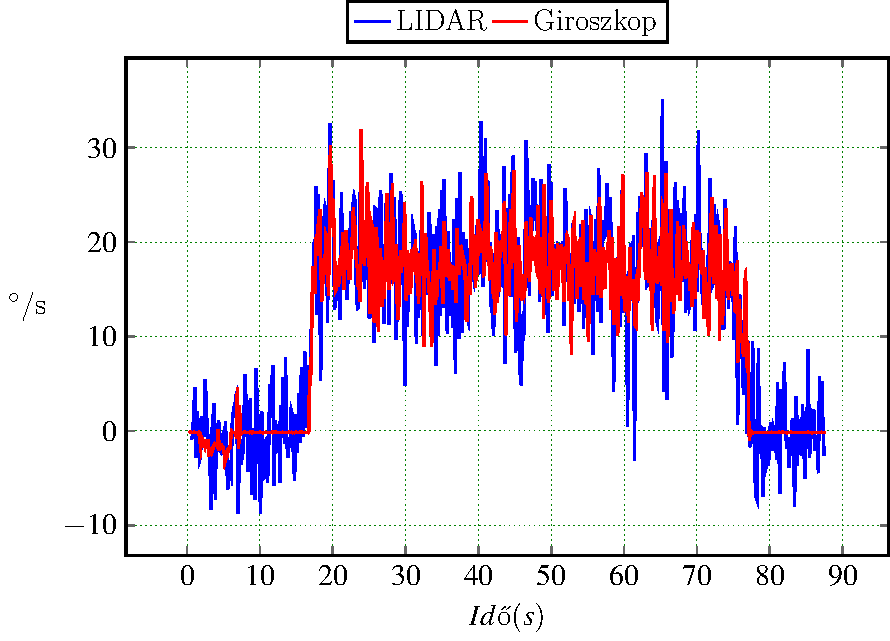
\includegraphics{tikz/Left_n50Right50d.pdf}
  \caption{$SSMR-4W$ típusú robot fordulási szögsebessége Z tengely körül, ha a kerekszőgsebességek BL=FL=50\degree/s és a FR=BR=-50\degree/s}
    \label{fig:Left_n50Right50d}
\end{figure}









